\documentclass{article}

\usepackage[T1]{fontenc}
\usepackage{libertine}

\usepackage{fancyhdr}
\usepackage{extramarks}
\usepackage{amsmath}
\usepackage{amsthm}
\usepackage{amsfonts}
\usepackage{tikz}
\usepackage{algorithm}
\usepackage{algpseudocode}
\usepackage{enumitem}

\usetikzlibrary{automata,positioning}

%
% Basic Document Settings
%

\topmargin=-0.45in
\evensidemargin=0in
\oddsidemargin=0in
\textwidth=6.5in
\textheight=9.0in
\headsep=0.25in

\linespread{1.1}

\pagestyle{fancy}
\lhead{\hmwkAuthorName}
\chead{\hmwkClass: \hmwkTitle}
\rhead{\firstxmark}
\lfoot{\lastxmark}
\cfoot{\thepage}

\renewcommand\headrulewidth{0.4pt}
\renewcommand\footrulewidth{0.4pt}

\setlength\parindent{0pt}

%
% Create Problem Sections
%

\newcommand{\enterProblemHeader}[1]{
    \nobreak\extramarks{}{Problem \arabic{#1} continued on next page\ldots}\nobreak{}
    \nobreak\extramarks{Problem \arabic{#1} (continued)}{Problem \arabic{#1} continued on next page\ldots}\nobreak{}
}

\newcommand{\exitProblemHeader}[1]{
    \nobreak\extramarks{Problem \arabic{#1} (continued)}{Problem \arabic{#1} continued on next page\ldots}\nobreak{}
    \stepcounter{#1}
    \nobreak\extramarks{Problem \arabic{#1}}{}\nobreak{}
}

\setcounter{secnumdepth}{0}
\newcounter{partCounter}
\newcounter{homeworkProblemCounter}
\setcounter{homeworkProblemCounter}{1}
\nobreak\extramarks{Problem \arabic{homeworkProblemCounter}}{}\nobreak{}

%
% Homework Problem Environment
%
% This environment takes an optional argument. When given, it will adjust the
% problem counter. This is useful for when the problems given for your
% assignment aren't sequential. See the last 3 problems of this template for an
% example.
%
\newenvironment{homeworkProblem}[1][-1]{
    \ifnum#1>0
        \setcounter{homeworkProblemCounter}{#1}
    \fi
    \section{Problem \arabic{homeworkProblemCounter}}
    \setcounter{partCounter}{1}
    \enterProblemHeader{homeworkProblemCounter}
}{
    \exitProblemHeader{homeworkProblemCounter}
}

%
% Homework Details
%   - Title
%   - Due date
%   - Class
%   - Section/Time
%   - Instructor
%   - Author
%

\newcommand{\hmwkTitle}{Homework\ \#2}
\newcommand{\hmwkDueDate}{February 15, 2018}
\newcommand{\hmwkClass}{Design and Analysis of Algorithms}
\newcommand{\hmwkClassInstructor}{Professor Kasturi Varadarajan}
\newcommand{\hmwkAuthorName}{\textbf{Alic Szecsei}}

%
% Title Page
%

\title{
    \vspace{2in}
    \textmd{\textbf{\hmwkClass:\ \hmwkTitle}}\\
    \normalsize\vspace{0.1in}\small{Due\ in\ class\ on\ \hmwkDueDate}\\
    \vspace{0.1in}\large{\textit{\hmwkClassInstructor}}
    \vspace{3in}
}

\author{\hmwkAuthorName}
\date{}

\renewcommand{\part}[1]{\textbf{\large Part \Alph{partCounter}}\stepcounter{partCounter}\\}

%
% Various Helper Commands
%

% Useful for algorithms
\newcommand{\alg}[1]{\textsc{\bfseries \footnotesize #1}}

% For derivatives
\newcommand{\deriv}[1]{\frac{\mathrm{d}}{\mathrm{d}x} (#1)}

% For partial derivatives
\newcommand{\pderiv}[2]{\frac{\partial}{\partial #1} (#2)}

% Integral dx
\newcommand{\dx}{\mathrm{d}x}

% Alias for the Solution section header
\newcommand{\solution}{\textbf{\large Solution}}

% Probability commands: Expectation, Variance, Covariance, Bias
\newcommand{\E}{\mathrm{E}}
\newcommand{\Var}{\mathrm{Var}}
\newcommand{\Cov}{\mathrm{Cov}}
\newcommand{\Bias}{\mathrm{Bias}}

% Set from 1 to N
\newcommand{\XYZ}[1]{\left\{1,\ldots,{#1}\right\}}
\newcommand{\Break}{\textbf{break} }

\begin{document}

\maketitle

\pagebreak

\begin{homeworkProblem}
Suppose we are given an array $A[1..n]$ with the special property that $A[1] \geq A[2]$ and $A[n-1] \leq A[n]$. We say that an element $A[x]$ is a \emph{local minimum} if it is less than or equal to both its neighbors, or more formally, if $A[x-1] \geq A[x]$ and $A[x] \leq A[x+1]$. For example, there are six local minima in the following array:\\
\begin{table}[h]
	\centering
	\begin{tabular}{ | *{15}{c |} c | }
		\hline
		9 & \textbf{7} & 7 & 2 & \textbf{1} & 3 & 7 & 5 & \textbf{4} & 7 & \textbf{3} & \textbf{3} & 4 & 8 & \textbf{6} & 9 \\
		\hline
\end{tabular}
	\caption{Example array}
	\label{tab:ExampleArray}
\end{table}

We can obviously find a local minimum in $O(n)$ time by scanning through the array. Describe and analyze an algorithm that finds a local minimum in $O(\log n)$ time. \emph{[Hint: With the given boundary conditions, the array \textbf{must} have at least one local minimum. Why?]}\\

\solution

\begin{algorithm}
	\caption{Algorithm for finding a local minimum}
	\label{algo:LocalMinimum}
	\begin{algorithmic}[1]
		\Function{FindLocalMinimum}{$A[1..n]$}
			\State{$median \gets n/2$}
			\If{$A[median] > A[median-1]$}
				\State{\Return{\Call{FindLocalMinimum}{$A[1..n/2]$}}}
			\ElsIf{$A[median] > A[median+1]$}
				\State{\Return{\Call{FindLocalMinimum}{$A[n/2..n]$}}}
			\Else{}
				\State{\Return{$median$}}
			\EndIf{}
		\EndFunction{}
	\end{algorithmic}
\end{algorithm}

Given the boundary conditions, the array \textbf{must} have at least one local minimum. To prove this, we can assume that the array has no local minimum. This means that the array must be either always increase or always decrease throughout the array; formally, $\forall x \in \XYZ{n}$, $A[x] > A[x-1]$ or $\forall x \in \XYZ{n}$, $A[x] > A[x+1]$. However since $A[1] \geq A[2]$ and $A[n-1] \leq A[n]$, this cannot be true; specifically it must \emph{start} by decreasing such that $A[x-1] \geq A[x]$ and then, at some point, start increasing, such that $A[x] \leq A[x+1]$. This point is the local minimum, since $A[x-1] \geq A[x] \leq A[x+1]$.\\

Given some median point, $m$, we can detect whether our array is increasing or decreasing at that point by examining the neighboring points. If the array is increasing, $A[m] \geq A[m-1]$. We know that the array starts by decreasing, so it must have started increasing since then; thus we can narrow our search for the local minimum to the first half of the array.\\

If the array is decreasing, $A[m] \geq A[m+1]$. Since the array ends with an increase, we know it must start increasing at some point after the median; thus we can narrow our search to the last half of the array.\\

If neither of these options is true, we must be at either a local maximum or minimum. If we are at a local maximum, then $A[m] \geq A[m-1]$, so we simply search the first half of the array; if we are at a local minimum, $A[m] \not> A[m+1]$ and $A[m] \not> A[m-1]$, so we reach our final branch and simply return $m$.

\end{homeworkProblem}

\pagebreak

\begin{homeworkProblem}
Suppose we are given two sorted arrays $A[1..n]$ and $B[1..n]$ and an integer $k$. Describe an algorithm to find the $k$th smallest element in the union of $A$ and $B$ in $\Theta(\log n)$ time. For example, if $k = 1$, your algorithm should return the smallest element of $A \cup B$; if $k = n$, your algorithm should return the median of $A \cup B$. You can assume that the arrays contain no duplicate elements. \emph{[Hint: First solve the special case $k = n$.]}\\

\solution

\begin{algorithm}
	\caption{Algorithm for finding the $k$th smallest element in a union}
	\label{algo:kthSmallest}
	\begin{algorithmic}[1]
		\Function{FindKSmallest}{$A[1..m], B[1..n], k$}
			\If{$k = 1$}
				\If{$m = 0$}
					\State{\Return{$B[1]$}}
				\ElsIf{$n = 0$}
					\State{\Return{$A[1]$}}
				\Else{}
					\State{\Return{$min(A[1], B[1])$}}
				\EndIf{}
			\Else{}
				\State{$mid \gets \left\lfloor \frac{k}{2} \right\rfloor$}
				\If{$mid \geq m + 1$}
					\State{\Call{FindKSmallest}{$A, B[mid+1..n], k - mid$}}
				\ElsIf{$mid \geq n + 1$}
					\State{\Call{FindKSmallest}{$A[mid+1..m], B, k - mid$}}
				\ElsIf{$A[mid] < B[mid]$}
					\State{\Call{FindKSmallest}{$A[mid+1..m], B, k - mid$}}
				\Else{}
					\State{\Call{FindKSmallest}{$A, B[mid+1..n], k - mid$}}
				\EndIf{}
			\EndIf{}
		\EndFunction{}
	\end{algorithmic}
\end{algorithm}

As an example, we will run through the algorithm with $A = \{1, 3, 5, 7\}$ and $B = \{2, 4, 6, 8\}$, with $k = 4$.\\

Since $k \neq 1$, we determine a middle element, $mid = \left\lfloor \frac{k}{2} \right\rfloor = 2$. Since $mid < m + 1$ and $mid < n + 1$, we compare the second element of each array. $A$ has a smaller element, since $A[2] = 3 < B[2] = 4$, so we recurse with a new $A = \{5, 7\}$, $B$ remaining the same, and $k = k - mid = 4 - 2 = 2$.\\

$k$ is still not $1$, so we determine our middle element, $mid = \left\lfloor \frac{k}{2} \right\rfloor = 1$. Since $mid < m + 1$ and $mid < n + 1$, we compare the first element of each array. $B$ has a smaller element, since $B[1] = 2$, so we recurse with a new $B = \{4, 6, 8\}$, $A$ remaining the same, and $k = k - mid = 2 - 1 = 1$.\\

Now, $k = 1$. Since neither $A$ nor $B$ are empty, we simply find the minimum of their first elements; $B[1] = 4$ and $A[1] = 5$, so we return $4$, as expected.\\

In general, we can divide the two arrays into four sections: $A_1$, $A_2$, $B_1$, and $B_2$, such that $A_1$ and $B_1$ have length $\frac{k}{2}$. Since we are looking for the $k$th smallest element, there are $k-1$ smaller elements we wish to discard. Let us define $A_{1_M}$ to be the largest element in $A_1$ and $B_{1_M}$ to be the largest element in $B_1$.\\

Let us first suppose that the $k$th smallest element is in either $A_1$ or $B_1$; without loss of generality, suppose it is in $A_1$. Then, since $\left| A_1 \cup B_1 \right| = k$, we know that up to $\frac{k}{2} - 1$ of the $k-1$ smaller elements are also in $A_1$. Therefore, there must be at least $\frac{k}{2}$ of the $k-1$ smaller elements in $B_1$. By definition, the $k$th smallest element will be larger than any of the $k-1$ smaller elements, so $A_{1_M} > B_{1_M}$, and our algorithm can safely remove $B_1$, as we know it contains only elements that are smaller than the $k$th smallest element.\\

Alternatively, we can suppose that the $k$th smallest element is in either $A_2$ or $B_2$; without loss of generality, suppose it is in $A_2$. Then, $A_1$ must contain $\frac{k}{2}$ of the $k-1$ smaller elements, since $A_1$ and $B_1$ contain $\frac{k}{2}$ elements. The opposite array ($B_1$) must therefore contain fewer than $\frac{k}{2}$ of the $k-1$ smaller elements, and will therefore have its largest element $B_{1_M}$ be greater than $A_{1_M}$; our algorithm then safely removes $A_1$, as we know it contains only elements that are smaller than the $k$th smallest element.\\

Since we have discarded elements smaller than the $k$th smallest, we update our value of $k$, removing the number of elements we discarded - $\frac{k}{2}$. We continue in this manner, discarding elements when possible, until we have reached our trivial base case, where $k = 1$ and we can simply find the minimal element of $A \cup B$.

\end{homeworkProblem}

\pagebreak

\begin{homeworkProblem}
For this problem, a \emph{subtree} of a binary tree means any connected subgraph. A binary tree is \emph{complete} if every internal node has two children, and every leaf has exactly the same depth. Describe and analyze a recursive algorithm to compute the \emph{largest complete subtree} of a given binary tree. Your algorithm should return the root and the depth of this subtree.

\begin{figure}[h]
	\centering
		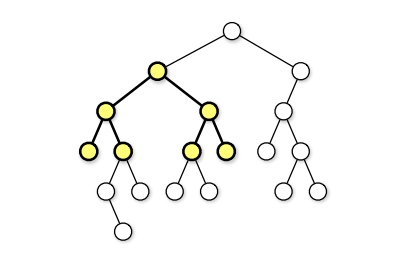
\includegraphics{images/binary-subtree.png}
	\caption{The largest complete subtree of this binary tree has depth 2.}
	\label{fig:binary-subtree}
\end{figure}

\solution\\

\begin{algorithm}
	\caption{Algorithm for finding the largest complete subtree}
	\label{algo:largestcomplete}
	\begin{algorithmic}[1]
		\Function{LargestCompleteSubtreeAt}{$node$}
			\If{$node.left$ exists and $node.right$ exists}
				\State{$childDepth \gets $ the minimum of \Call{LargestCompleteSubtreeAt}{$node.left$} and \Call{LargestCompleteSubtreeAt}{$node.right$}}
				\State{\Return{$1 + childDepth$}}
			\Else{}
				\State{\Return{0}}
			\EndIf{}
		\EndFunction{}
		\Function{LargestCompleteSubtreeAt}{$root$}
			\State{$rootDepth \gets$ \Call{LargestCompleteSubtreeAt}{$root$}}
			\If{$node.left$ exists}
				\State{$leftDepth, leftNode \gets$ \Call{LargestCompleteSubtree}{$node.left$}}
			\EndIf{}
			\If{$node.right$ exists}
				\State{$rightDepth, rightNode \gets$ \Call{LargestCompleteSubtree}{$node.left$}}
			\EndIf{}
			\State{$maxDepth \gets$ the maximum of $rootDepth$, $leftDepth$, and $rightDepth$}
			\If{$maxDepth = rootDepth$}
				\State{\Return{$maxDepth, root$}}
			\ElsIf{$maxDepth = leftDepth$}
				\State{\Return{$maxDepth, leftNode$}}
			\Else{}
				\State{\Return{$maxDepth, rightNode$}}
			\EndIf{}
		\EndFunction{}
	\end{algorithmic}
\end{algorithm}

Our first function exists to determine the largest complete subtree beginning at a particular node. This way, we can separate our concerns to aid with recursion. Our second function repeatedly calls the first function to determine the largest complete subtree at any position in the tree; we do this by recursing through it and finding the largest complete subtree starting from every node in the tree.\\

The run-time of \alg{LargestCompleteSubtreeAt} has a recurrence of $T_1(n) = 2T_1(\frac{n}{2}) + 1$. Using the Master Theorem, we can solve this recurrence:

\begin{equation}
\begin{split}
a & = 2\\
f(\frac{n}{b}) &= 1\\
f(n) &= 1\\
a f(\frac{n}{b}) &= K f(n)\\
2 \times 1 &= K \times 1\\
K &= 2
\end{split}
\end{equation}

Since $K > 1$, the Master Theorem states that $T_1(n) = \Theta(n^{\log_b a})$; with $b = 2$ and $a = 2$, we get $T_1(n) = \Theta(n^{\log_2 2})$, which trivially reduces to $T_1(n) = \Theta(n^1) = \Theta(n)$.\\

The unoptimized run-time of \alg{LargestCompleteSubtree} has a recurrence of $T_2(n) = 2T_2(\frac{n}{2}) + T_1(n)$. Using the Master Theorem, we get:

\begin{equation}
\begin{split}
a &= 2\\
f(\frac{n}{b}) &= \frac{n}{2}\\
f(n) &= n\\
a f(\frac{n}{b}) &= K f(n)\\
2 \frac{n}{2} &= K \times n\\
K &= 1
\end{split}
\end{equation}

Since $K = 1$, the Master Theorem states that $T_2(n) = \Theta(f(n)\log_b n)$, so $T_2(n) = \Theta(n\log_2 n)$.\\

This could easily be optimized with memoization; we can cache the results of \alg{LargestCompleteSubtreeAt}. In this case, no repeated calculations of \alg{LargestCompleteSubtreeAt} occur, so rather than running in $\Theta(n\log_2 n)$, it would run in $\Theta(n)$.

\end{homeworkProblem}

\pagebreak

\begin{homeworkProblem}
A \emph{sequence of integers} is either empty or an integer followed by a sequence of integers.\\

The only \emph{subsequence} of the empty sequence is the empty sequence.\\

A \emph{subsequence} of $A[1..n]$ is either a subsequence of $A[2..n]$ or $A[1]$ followed by a subsequence of $A[2..n]$.\\

\begin{enumerate}[label=(\alph*)]
	\item Let $A[1..m]$ and $B[1..n]$ be two arbitrary arrays. A \emph{common subsequence} of $A$ and $B$ is both a subsequence of $A$ and a subsequence of $B$. Give a simple recursive definition for the function $lcs(A,B)$, which gives the length of the \emph{longest} common subsequence of $A$ and $B$.
	\item Call a sequence $X[1..n]$ \emph{oscillating} if $X[i] < X[i+1]$ for all even $i$, and $X[i] > X[i+1]$ for all odd $i$. Give a simple recursive definition for the function $los(A)$, which gives the length of the longest oscillating subsequence of an arbitrary array $A$ of integers.
	\item Call a sequence $X[1..n]$ \emph{accelerating} if $2 \times X[i] < X[i-1] + X[i+1]$ for all $i$. Give a simple recursive definition for the function $lxs(A)$, which gives the length of the longest accelerating subsequence of an arbitrary array $A$ of integers.
\end{enumerate}

\solution\\

\part

\begin{algorithm}
	\caption{Algorithm for finding the length of the longest common subsequence}
	\label{algo:longestcommon}
	\begin{algorithmic}[1]
		\Function{LCS}{$A[1..m], B[1..n]$}
			\If{$m = 0$ or $n = 0$}
				\State{\Return{0}}
			\Else{}
				\State{$a \gets$ \Call{LCS}{$A[2..m], B[1..n]$}}
				\State{$b \gets$ \Call{LCS}{$A[1..m], B[2..n]$}}
				\State{$c \gets 0$}
				\If{$A[1] = B[1]$}
					\State{$c \gets 1 +$ \Call{LCS}{$A[2..m], B[2..n]$}}
				\EndIf{}
				\State{$r \gets$ the maximum of $a$, $b$, and $c$}
			\EndIf{}
		\EndFunction{}
	\end{algorithmic}
\end{algorithm}

This is the simplest of the three sections; we simply provide 3 options for the algorithm. The longest common subsequence may lie further down $A$, further down $B$, or include the first values of both $A$ and $B$ - though this third option is only valid if $A$ and $B$ both have the same first values. The algorithm calculates all three routes, and compares the results at the end to determine the correct result.

\pagebreak
\part

\begin{algorithm}
	\caption{Algorithm for finding the length of the longest oscillating subsequence}
	\label{algo:longestosc}
	\begin{algorithmic}[1]
		\Function{LOS}{$X[1..n]$}
			\State{\Return{\Call{LOS2}{$X[1..n], null, false$}}}
		\EndFunction{}
		\Function{LOS2}{$X[1..n], prevValue, isEven$}
			\If{$n = 0$}
				\State{\Return{$0$}}
			\Else{}
				\If{$prevValue = null$}
					\State{$result \gets true$}
				\ElsIf{$isEven$}
					\State{$result \gets prevValue > X[1]$}
				\Else{}
					\State{$result \gets prevValue < X[1]$}
				\EndIf{}
				
				\State{$a \gets$ \Call{LOS2}{$X[2..n], prevValue, isEven$}}
				\If{$result$}
					\State{$b \gets 1 +$ \Call{LOS2}{$X[2..n], X[1],$ not $isEven$}}
				\Else{}
					\State{$b \gets 0$}
				\EndIf{}
				\State{\Return{the maximum of $a$ and $b$}}
			\EndIf{}
		\EndFunction
	\end{algorithmic}
\end{algorithm}

For this solution, we need a helper function to keep track of whether the sequence should be increasing or decreasing, as well as what the previous entry in the sequence was.\\

First we check the length of the array, as a base case. Then, we try skipping the current entry, in the $a$ path.\\

Finally, we determine if the current entry is acceptable. If there was no prior entry, then we can use the current entry; otherwise, we must check whether the current entry is increasing or decreasing compared to the prior entry. If the current entry is acceptable, we attempt to continue the sequence in the $b$ path.\\

Once both the $a$ and $b$ paths have been considered, we simply return the larger of the two results.

\pagebreak
\part

\begin{algorithm}
	\caption{Algorithm for finding the length of the longest accelerating subsequence}
	\label{algo:longestaccel}
	\begin{algorithmic}[1]
		\Function{LXS}{$X[1..n]$}
			\State{\Return{\Call{LXS2}{$X[1..n], null, null$}}}
		\EndFunction{}
		\Function{LXS2}{$X[1..n], prevValue, prevDiff$}
			\If{$n = 0$}
				\State{\Return{$0$}}
			\Else{}
				\If{$prevValue = null$ or $prevDiff = null$}
					\State{$result \gets true$}
				\Else{}
					\State{$result \gets X[1] - prevValue > prevDiff$}
				\EndIf{}
				\State{$a \gets$ \Call{LXS2}{$X[2..n], prevValue, prevDiff$}}
				\If{$result$}
					\If{$prevValue = null$}
						\State{$b \gets 1 +$ \Call{LXS2}{$X[2..n], X[1], null$}}
					\Else{}
						\State{$b \gets 1 +$ \Call{LXS2}{$X[2..n], X[1], X[1] - prevValue$}}
					\EndIf{}
				\Else{}
					\State{$b \gets 0$}
				\EndIf{}
				\State{\Return{the maximum of $a$ and $b$}}
			\EndIf{}
		\EndFunction{}
	\end{algorithmic}
\end{algorithm}

Similar to the previous problem, we use a helper function to keep track of the previous value in the sequence ($X[i]$, as well as the previous difference in values; that is, $X[i] - X[i-1]$.\\

Again, we calculate an $a$ path in which we skip the current value in $X$; then we calculate a $B$ path if either:

\begin{enumerate}
	\item There was no prior value (the first entry in the subsequence)
	\item There was no prior difference in values (The second entry in the subsequence)
	\item The current value satisfies the properties of an accelerating subsequence, so that $X[i+1] - X[i] > X[i] - X[i-1]$.
\end{enumerate}

If any of these are true, then the current value of $X$ is a viable addition to the sequence. Finally, we compare the results of the $a$ and $b$ paths to determine which is larger.

\end{homeworkProblem}

\end{document}